
\documentclass{beamer}

\usetheme{Madrid}
\usepackage{indentfirst} 
\usepackage{graphicx} 
\usepackage{booktabs}
\usepackage{amsmath}
\usepackage{setspace}
\usepackage{algorithm,algorithmic}
\usepackage{float}

\title{Immune Algorithm}

\author{2017 Spring OPT}

\institute[] 
{Shen,Zheng; Li,Meizhen; Cao,Jing; Shi,Haixin; Zhong,Wenfeng; Han,Shiqi}

\date{\today}

\AtBeginSubsection[]
{
  \begin{frame}<beamer>{Outline}
    \tableofcontents[currentsection,currentsubsection]
  \end{frame}
}

\begin{document}

\begin{frame}
  \titlepage
\end{frame}

\begin{frame}{Outline}
  \tableofcontents
\end{frame}

\section{General Immune Algorithm}

\begin{frame}
\Huge \textbf{General Immune Algorithm}
\large {Shen,Zheng}
\end{frame}

\begin{frame}{Biological principles of immune algorithm}{The working model of the immune system}
 
  
  \par
  \centering
  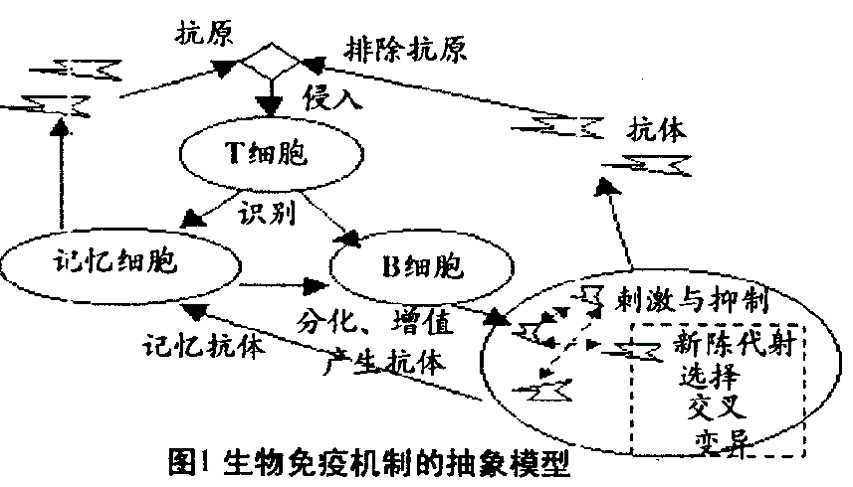
\includegraphics[scale=0.5]{img/1.png}
  \par
  
\end{frame}
\begin{frame}{Comparison of immune system and immune algorithm}
 
  
  \par
  \centering
  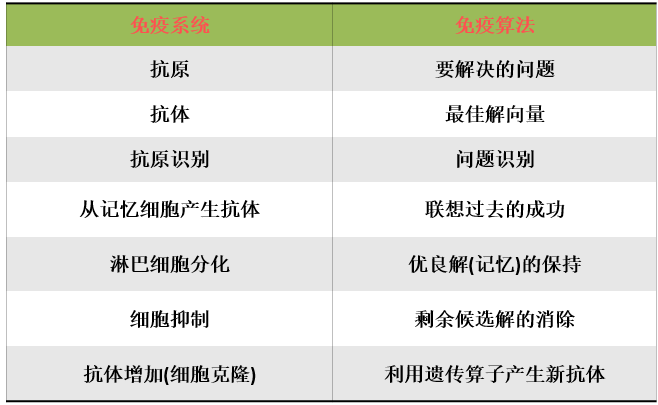
\includegraphics[scale=0.6]{img/2.PNG}
  \par
  
\end{frame}



\begin{frame}{Comparison of immune system and immune algorithm}
\par\setlength\parindent{9em}
Immune Operator:
 \par\setlength\parindent{11em}
 1.Full Immunity
 \par\setlength\parindent{11em}
 2.Target Immunity
    

     
 
\end{frame}


\begin{frame}{
Immune Operator}
\begin{block}{Full Immunity}
Full immunity refers to the type of immunity that each group of individuals in a group has an immune operation on every link after the action of genetic operators. It is mainly applied to the initial stage of individual evolution, but not in the process of evolution.
\end{block}
\begin{block}{Target Immunity}
The target immunity refers to a type of immune response at the point of action only after a genetic operation. The target immunization is generally associated with the whole process of population evolution, and it is a basic operator of the immune operation.
\end{block}

\end{frame}

\begin{frame}{Immune Algrithm}
 
 \indent 
 1.The specific analysis of the solved problems(regarded as an antigen)
 \newline
 2.This feature information is processed to transform it into a solution to the problem(The set of solutions obtained according to the scheme is called the antibody based on the vaccine above)
 \newline
 3.Transform this scheme into an immune operator in an appropriate form
 
\end{frame}

\begin{frame}{Immune algorithm based on genetic algorithm}
 
  
  \par
  \centering
  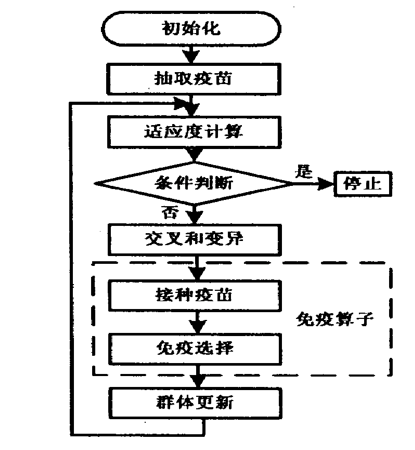
\includegraphics[scale=0.6]{img/5.PNG}
  \par
  
\end{frame}

\begin{frame}{Immune Operator}
 
 \indent 
 1.Vaccination:According to the prior knowledge, some genes in X are modified to make the individual have higher fitness for greater probability. 
 
 \newline
 
2.Immune selection:
\par\setlength\parindent{6em}
(1)Immunoassay:The detection of individuals vaccinated is not as good as the parent, indicating that the phenomenon of severe degeneration has occurred during the process of crossover and mutation, and this individual will be replaced by the corresponding individuals in the parent.
\par\setlength\parindent{6em}
(2)Annealing selection:
In the current progeny group E_k=(x_1,...,x_{n_0}), 

the individual Xi is selected by the probability $P(x_i)$ to enter the new parent group:
\par\setlength\parindent{6em}
P(x_i)=e^{f(x_i)/T_k}\sum_{i=1}^{n_0}e^{f(xi)/T_k}
\par\setlength\parindent{6em}
$f(x_i)$ is the adaptive degree of individual,
\par\setlength\parindent{6em}
$T_k$is a temperature control sequence approaching 0
 \newline
\end{frame}
\begin{frame}{Immune Operator}
 
 \indent 
$a_{H,k}^i$ is the antibody obtained after vaccinating the k generation the i individual $a_k^i$. $P_I$ is the probability of vaccinating individuals, and $P_V$ is the probability of updating the vaccine. $V(a_k^i,h_j)$ is an inoculation operation modifing the gene on an individual$a_k^i$ according to the pattern $h_j$,  and N and m are the size of the population and the vaccine, respectively.
 
 \newline
 

\par\setlength\parindent{6em}

\end{frame}

\begin{frame}{The execution algorithm of immune operator}
 
  \par\setlength\parindent{6em}
Begin:
\par\setlength\parindent{6em}
  Extraction of vaccine:
  \par\setlength\parindent{8em}
  Analyze the problem to be asked and collect the characteristic information
  \par\setlength\parindent{8em}
  Estimation of patterns on specific gene sites based on characteristic information:H={h_j|j=1,2,...,m}
   \par\setlength\parindent{6em}
   k=0andj=0;
   \par\setlength\parindent{6em}
   while(Conditions=true)
   \par\setlength\parindent{7em}
    if{P_v}=true,then j=j+1;
    \par\setlength\parindent{7em}
    i=0;
    \par\setlength\parindent{7em}
    for(i<=n)
    \par\setlength\parindent{8em}
    Vaccination:a_{H,k}^j=V_{p_I}{(a_k^i,h_j)};
    \par\setlength\parindent{8em}
    Immunoassay:if a_{H,k}^i<a_{k-1}^i,then a_k^j=a_{k-1}^i;
    else a_k^i=a_{H,k}^i;
    \par\setlength\parindent{8em}
    i=i+1;
    \par\setlength\parindent{7em}
    Annealing selection:A_{k+1}=S(A_k);
    \par\setlength\parindent{7em}
    k=k+1;
    
    End
  
  

  
\end{frame}




\section{Clonal Selection Algorithm}

\begin{frame}
\centering
\Huge \textbf{Clonal Selection Algorithm} 
\\
\large \rightline {Cao,Jing \quad}
\end{frame}

\begin{frame}{The Clonal Selection Theory}
\begin{itemize}
\item{1. B cell products antibodies(Ab) when an animal is exposed to an antigen;}
\item{2. Each B cell secrets only one kind of antibody, which is relatively specific for antigen;}
\item{3. The antigen stimulates the B cell to proliferate(divide) and mature into terminal (non-dividing) antibody secreting cells, called plasma cells;}
\end{itemize}
\end{frame}


\begin{frame}{The Clonal Selection Theory}
\begin{columns}[c] 
\column{.45\textwidth} 
\begin{itemize}
\item{4. Lymphocytes, in addition to proliferating and/or differentiating into plasma cells, can differentiate into long-lived B  memory cells;}
\item{5. When exposed to the same antigen again, the B memory cells can differentiate into large lymphocytes quickly to produce high affinity antibodies;}
\end{itemize}
\column{.55\textwidth} 
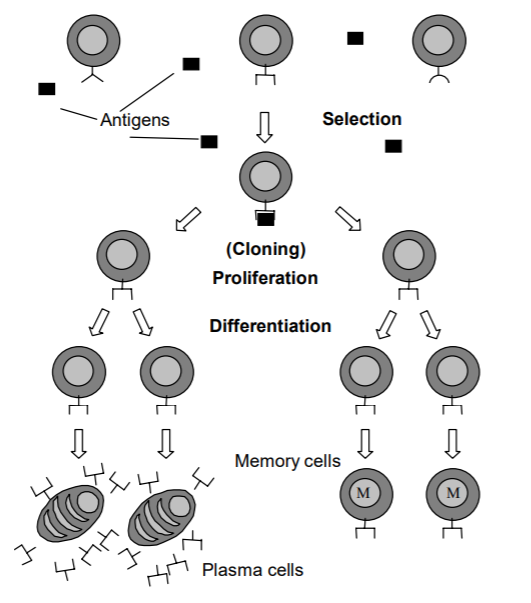
\includegraphics[height=6cm]{img/cj_clone_selection_p.png}
\end{columns}
\end{frame}

\begin{frame}{Reinforcement Learning and Memory}
\begin{columns}[c] 
\column{.45\textwidth}
\begin{itemize}
\item{1. The effectiveness of the immune response to secondary encounters is considerably enhanced  \textcolor{red}{by storing some high affinity antibody} producing cells from the first infection;}
\item{2. Such a strategy ensures that both the speed and accuracy of the immune response \textcolor{red}{becomes successively greater after each infection};}
\item{This scheme is intrinsic of a \textcolor{red}{reinforcement learning strategy} }
\end{itemize}
\column{.55\textwidth} 
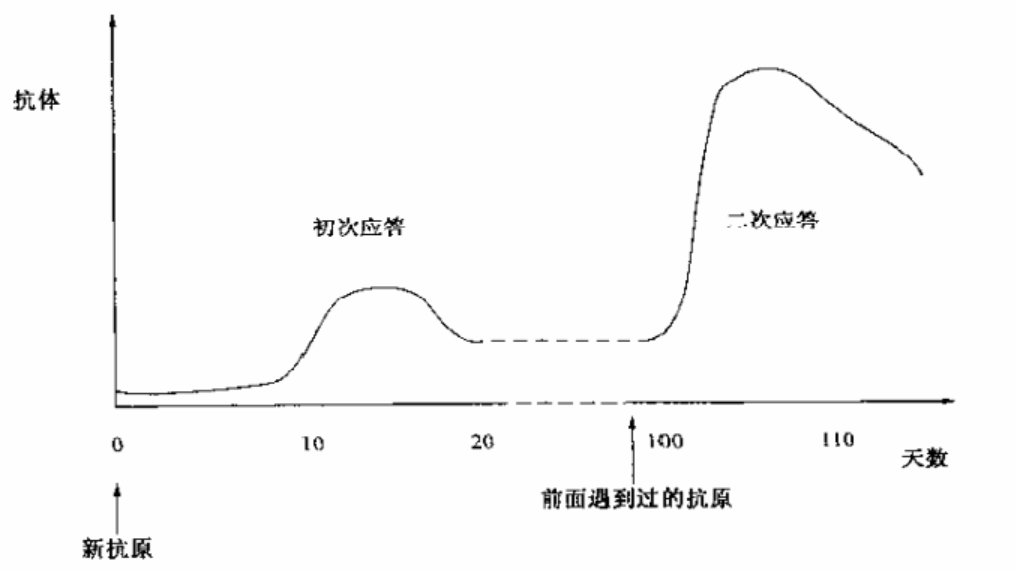
\includegraphics[height=4cm]{img/cj_reinfor_learn.png}
\end{columns}
\end{frame}


\begin{frame}{Reinforcement Learning and Memory}
\begin{itemize}
\item{One important characteristic of the immune memory is that it is associative: B cells adapted to a certain type of antigen A1 presents a faster and more efficient secondary response not only to A1, \textcolor{red}{but also to any structurally related antigen A2.  This phenomenon is called immunological cross-reaction, or cross-reactive response}.}
\item{Antibodies present in a memory response have, \textcolor{red}{on average, a higher affinity than those of the early primary response}. This phenomenon, is referred to as the maturation of the immune response}
\end{itemize}
\end{frame}


\begin{frame}{Somatic Hypermutation, Receptor Editing and Repertoire Diversity}
\begin{columns}[c] 
\column{.45\textwidth} 
\begin{itemize}
\item{1. Point mutations allow the immune system to explore local areas around A by making \textcolor{red}{small steps} towards an antibody with higher affinity;}
\item{2. Receptor editing allows an antibody to take \textcolor{red}{large steps} through the landscape, landing in a locale where the affinity might be lower;}
\end{itemize}
\column{.55\textwidth} 
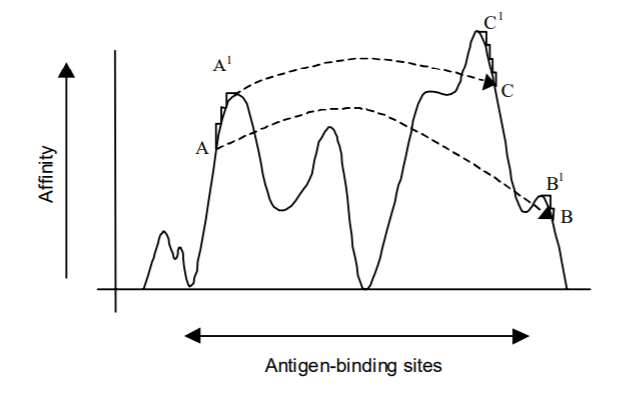
\includegraphics[height=4.5cm]{img/cj_somatic_muta.png}
\end{columns}
\end{frame}

\begin{frame}{The Regulation of the Hypermutation Mechanism}
\begin{itemize}
\item{1. The majority of the mutations  will lead to poorer or non-functional antibodies;}
\item{2. If a cell mutate at a fixed rate, the accumulation of deleterious changes may cause the loss of the advantageous mutation;}
\item{\textcolor{red}{So there should be a selection mechanism}}
\end{itemize}
\end{frame}


\begin{frame}{The Regulation of the Hypermutation Mechanism}
\begin{itemize}
\item{Cells with low affinity receptors may be further mutated and, as a rule, \textcolor{red}{die} if they do not become higher affinity cells. In cells with high-affinity antibody receptors however, hypermutation may be \textcolor{red}{inactivated}.}
\end{itemize}
\end{frame}

\begin{frame}{The Shape-Space Model}
\begin{itemize}
\item{1. The shape-space model (\begin{math} S\end{math}) aims at quantitatively describing the interactions among antigens and antibodies (be \textcolor{red}{Ag-Ab});}
\item{2. The set of features that characterize a molecule is called its \textcolor{red}{generalized shape};}
\item{
3. Mathematically, the generalized shape of a molecule (\begin{math} m\end{math}), either an antibody or an antigen, can be represented by a set of coordinates \begin{math} m =\left \langle m_1, m_2,..., m_L\right\rangle\end{math}, which can be regarded as a point in an \\
L-dimensional real-valued shape-space (m \in S^L);
}
\end{itemize}
\end{frame}



\begin{frame}{The Proposed Algorithm}
\begin{columns}[c] 
\column{.45\textwidth} 
\begin{itemize}
\item{After each six steps we have one cell generation}
\item{(1) Generate a set of (\begin{math} P \end{math}) of candidate solutions, composed of the subset of memory cells  (\begin{math} M \end{math}) added to the remaining (\begin{math} P_r \end{math}) population (\begin{math} P = P_r + M \end{math});}
\item{(2) Determine (Select) the n best individuals of population (\begin{math} P_n \end{math}), based on affinity measure;}
\end{itemize}
\column{.55\textwidth} 
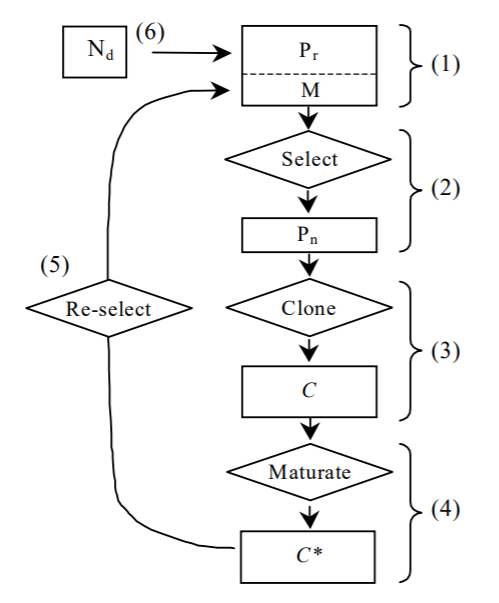
\includegraphics[height=6.5cm]{img/cj_block_diagram_CSA.png}
\end{columns}
\end{frame}


\begin{frame}{The Proposed Algorithm}
\begin{columns}[c] 
\column{.45\textwidth} 
\begin{itemize}
\item{(3) Reproduce (Clone) these n best individuals of the population, giving rise to a temporary population of clones (\begin{math} C \end{math}). The clone size is an increasing function of the affinity with the antigen;}
\item{(4) Submit the population of clones to a hypermutation scheme, where the hypermutation is proportional to the affinity of the antibody with the antigen. A maturated antibody population is generated (\begin{math} C^* \end{math});}
\end{itemize}
\column{.55\textwidth} 
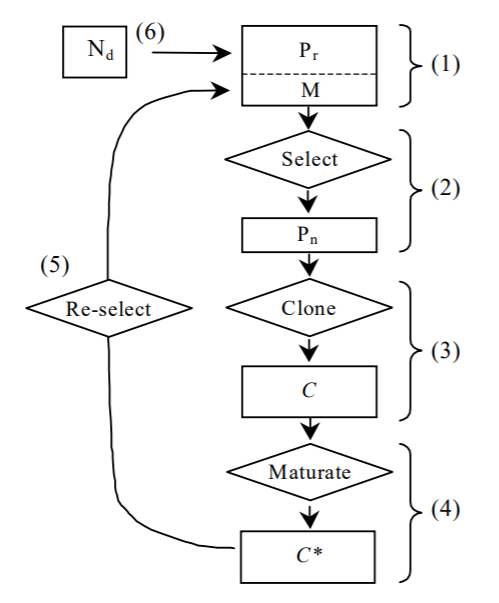
\includegraphics[height=6.5cm]{img/cj_block_diagram_CSA.png}
\end{columns}
\end{frame}


\begin{frame}{The Proposed Algorithm}
\begin{columns}[c] 
\column{.45\textwidth} 
\begin{itemize}
\item{(5) Re-select the improved individuals from \begin{math} C^* \end{math} to compose the memory set \begin{math} M \end{math}. Some members of \begin{math} P \end{math} can be replaced by other improved members of \begin{math} C^* \end{math};}
\item{(6) Replace \begin{math} d \end{math} antibodies by novel ones (diversity introduction). The lower affinity cells have higher probabilities of being replaced;}
\end{itemize}
\column{.55\textwidth} 
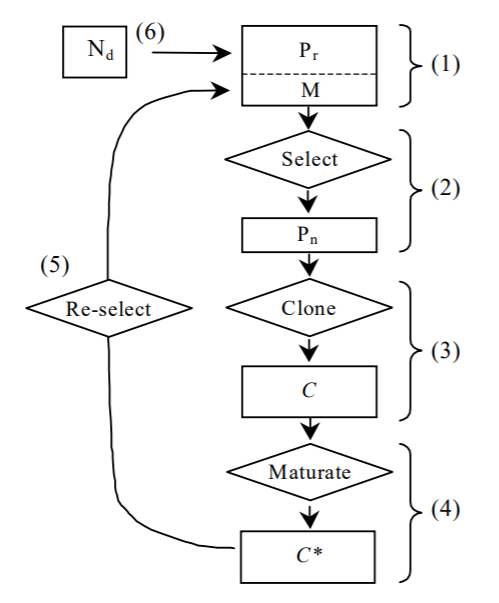
\includegraphics[height=6.5cm]{img/cj_block_diagram_CSA.png}
\end{columns}
\end{frame}

\begin{frame}{Engineering Applications}{Binary Character Recognition}
\begin{itemize}
\item{The goal is to demonstrate that a cumulative blind variation together with selection can \textcolor{red}{produce individuals with increasing affinities} (maturation of the immune response);}
\item{In this case, we assume that the antigen population is represented by a set of eight binary characters to be learned. ;}
\item{Each character is represented by a bitstring of length \begin{math} L = 120 \end{math};}
\end{itemize}

\includegraphics[height=1.5cm]{img/cj_bitsstring.png}
\end{frame}


\begin{frame}{Engineering Applications}{Binary Character Recognition}
\begin{itemize}
\item{The affinity measure takes into account the Hamming distance (\begin{math} D \end{math}) between antigens and antibodies, according to Equation (1):}
\begin{equation} \small{
 D =\sum_{i=1}^{L} \delta \quad where \  \delta = \begin{cases} 1 & \mbox{ if } \  ab_i \neq ag_i \\
 0  & otherwise \end{cases}}
 \end{equation}
\end{itemize}
\end{frame}

\begin{frame}{Engineering Applications}{Binary Character Recognition}
\begin{figure}[h]
\centering
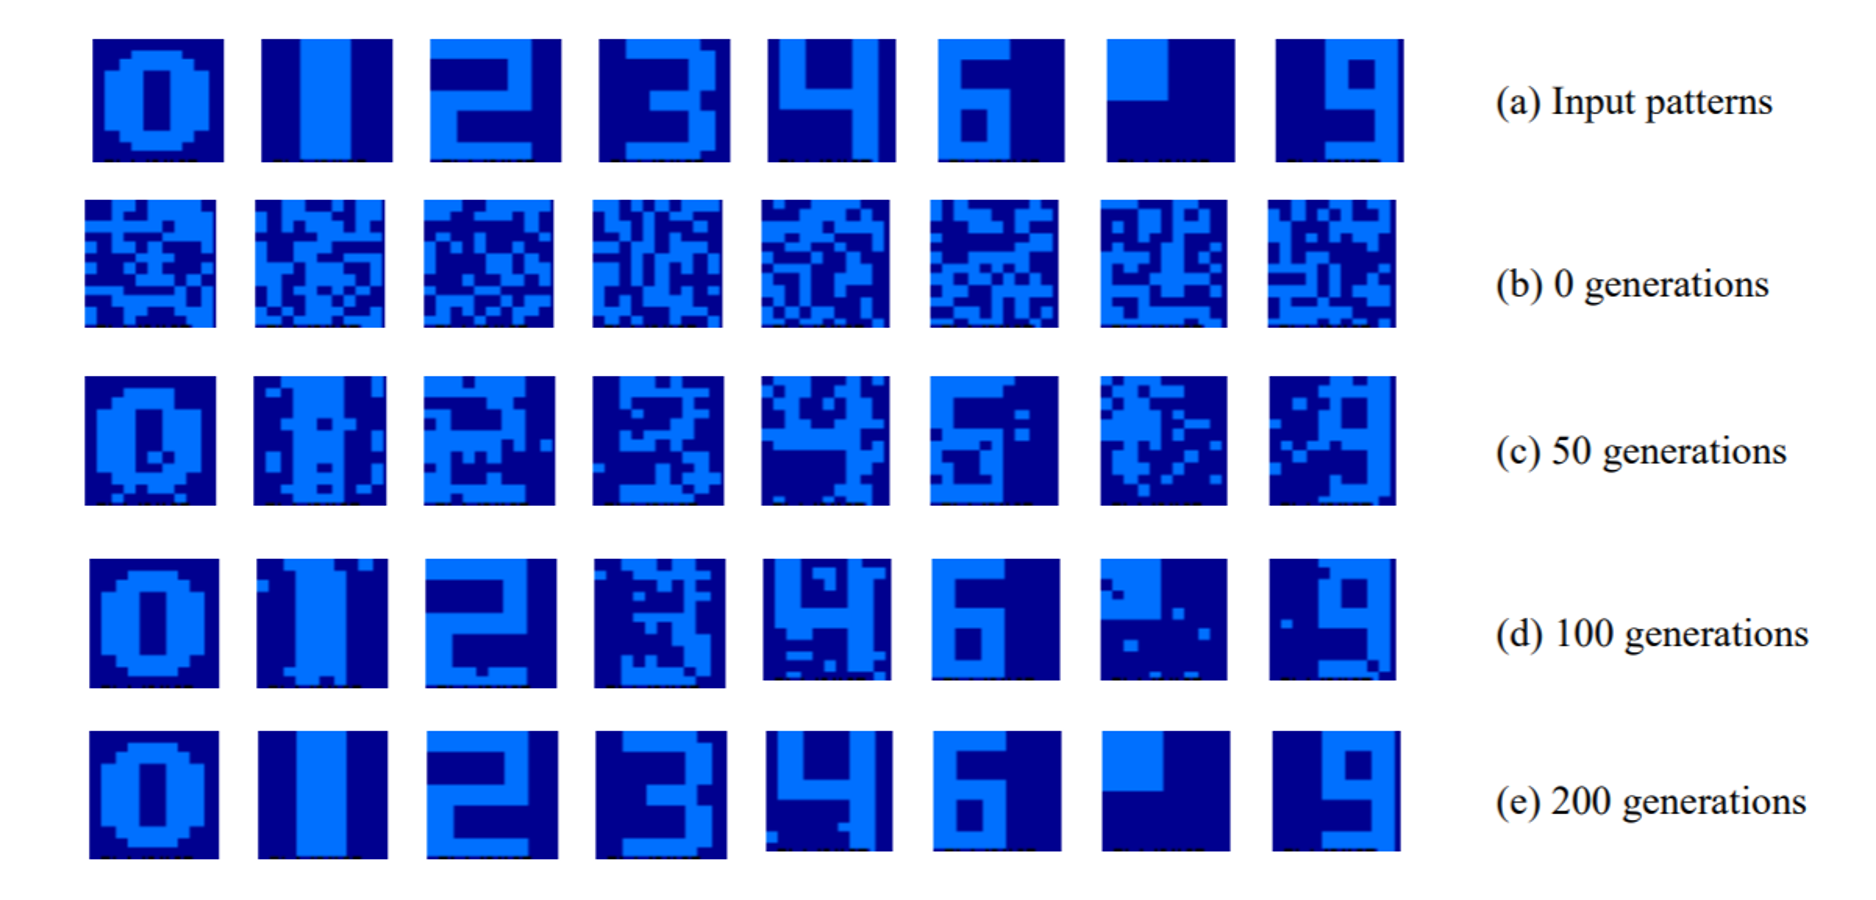
\includegraphics[height=6cm]{img/cj_binary_pattern_learn.png}
\end{figure}
\end{frame}


\begin{frame}{Engineering Applications}{Multi-Modal Optimization}
\begin{itemize}
\item{The CSA reproduces those individuals with higher affinities and selects their improved maturated progenies;} 
\item{This strategy suggests that the algorithm performs a greedy search, where single members will be locally optimized (exploitation of the surrounding space), and the newcomers yield a broader exploration of the searchspace;}
\item{This characteristic makes the CSA \textcolor{red}{very suitable for solving multi-modal optimization tasks}}
\end{itemize}
\end{frame}

\begin{frame}{Engineering Applications}{Multi-Modal Optimization}
\begin{itemize}
\item{Consider the maximizing the function:}
\begin{equation} \small{
f(x, y) = x \cdot sin(4 \pi x) - y \cdot sin(4 \pi y + \pi) +1}
 \end{equation}
\end{itemize}
\begin{figure}[h]
\centering
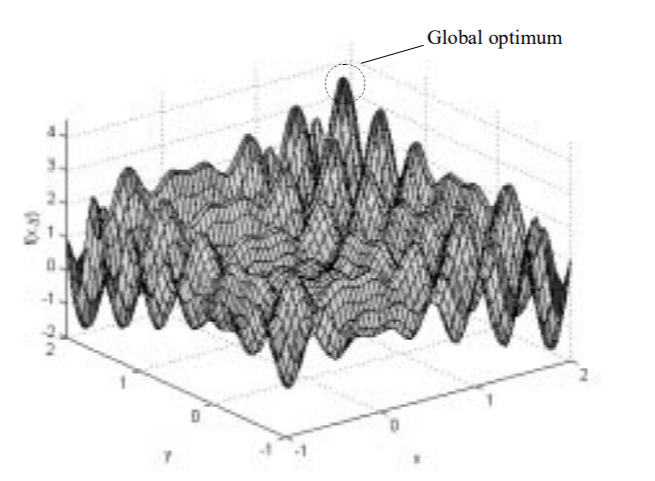
\includegraphics[height=5.5cm]{img/cj_func_maxi.png}
\end{figure}
\end{frame}


\begin{frame}{Engineering Applications}{Multi-Modal Optimization}
\begin{itemize}
\item{We employed the Hamming shape-space, with binary strings representing real values for \begin{math} x \end{math} and \begin{math} y \end{math};}
\item{The chosen bitstring length was \begin{math} L = 22 \end{math},  corresponding to a precision of six decimal places}
\item{The variables \begin{math} x \end{math} and \begin{math} y \end{math} are defined over the range \begin{math} [-1, 2]\end{math},  and the mapping from a binary string  \begin{math} m =\left \langle m_L,..., m_2, m_1\right\rangle\end{math} into a real number \begin{math} z \end{math} is completed in two steps:}
\begin{itemize}
    \item {convert the binary string \begin{math} m =\left \langle m_L,..., m_2, m_1\right\rangle\end{math} from base 2 to base 10:}
    \begin{equation}\small{(<m_L,..., m_2, m_1>)_2 = (\sum_{i=0}^{21}m_i \cdot 2^i)_{10} \ = \ z^{'}}
    \end{equation}
    \item{find the corresponding real value for \begin{math} z \end{math}:}
    \begin{equation}\small{z=z_{min} + z^{'} \cdot \frac{z_{max} - z_{min}}{2^{22} - 1}, \ where \ z_{max} = 2 \ and \ z_{min} = -1
    }
    \end{equation}
\end{itemize}
\end{itemize}
\end{frame}


\begin{frame}{Engineering Applications}{Multi-Modal Optimization}
\begin{itemize}
\item{The affinity measure corresponds to the evaluation of the
function \begin{math} f(x, y) \end{math} after decoding \begin{math} x \end{math} and \begin{math} y \end{math}, as described above;}
\item{The figure below present the  optimized population after 100
generations:}
\end{itemize}
\begin{figure}[h]
\centering
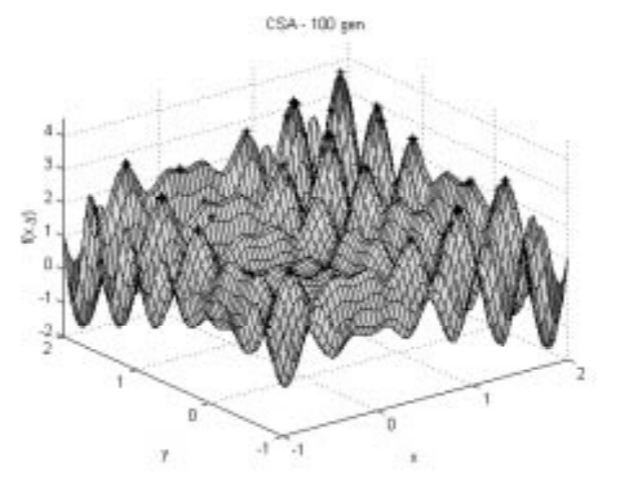
\includegraphics[height=5.5cm]{img/cj_func_maxi_100.png}
\end{figure}
\end{frame}

\begin{frame}{Engineering Applications}{Multi-Modal Optimization}
\begin{itemize}
\item{Notice that the solutions (stars) covers most of the peaks, including the global optimum. }
\end{itemize}
\begin{figure}[h]
\centering
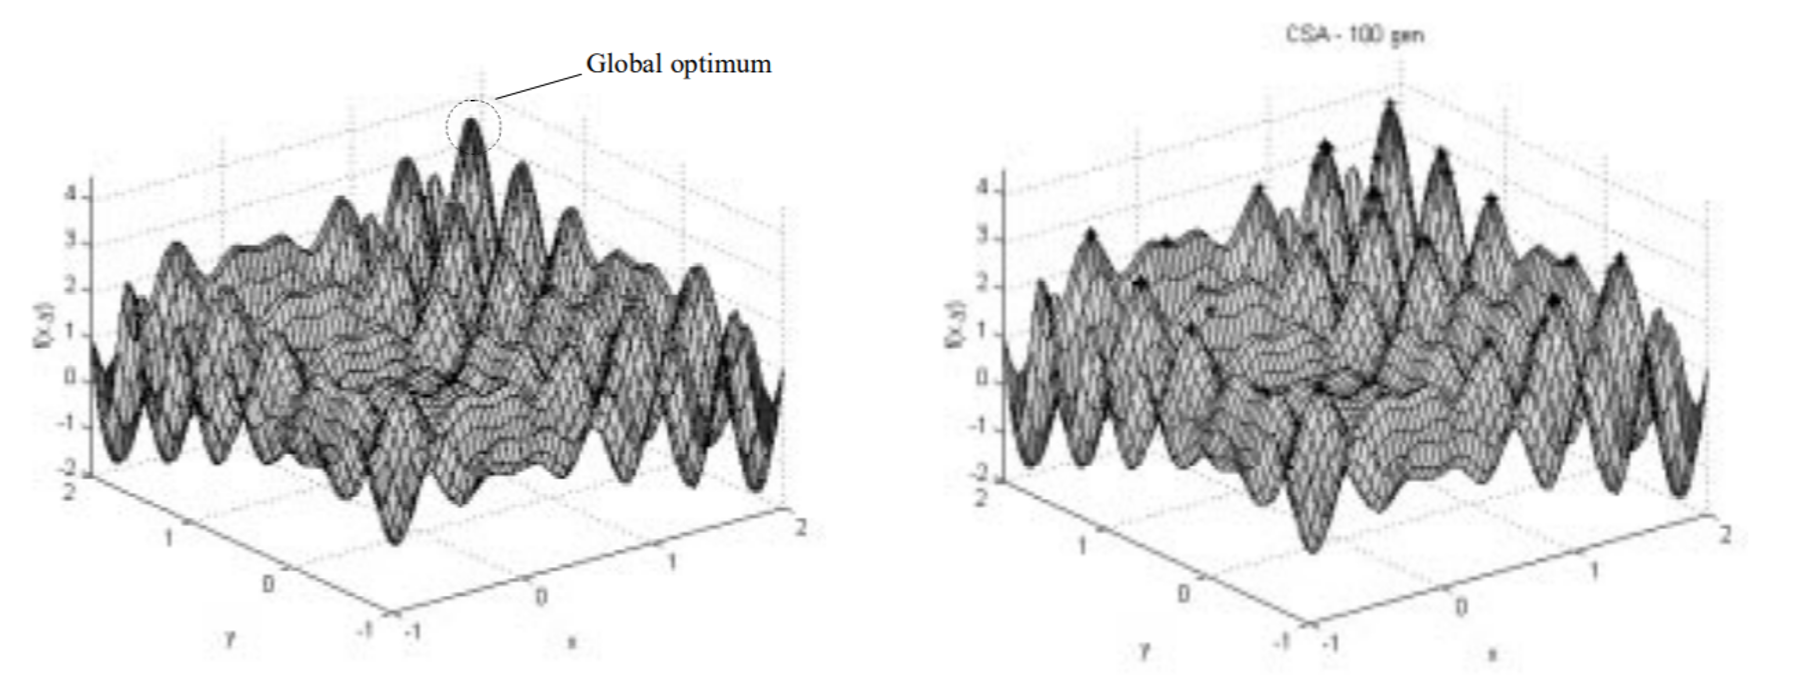
\includegraphics[height=4.5cm]{img/cj_func_and.png}
\end{figure}
\end{frame}


\begin{frame}{Conclusion}
\begin{itemize}
\item{The algorithm was verified to be capable of performing learning and maintenance of high quality memory and, it was also capable of solving complex problems, like multi-modal and combinatorial optimization.}
\end{itemize}

\end{frame}

\section{Negative Selection Algorithm}

\begin{frame}{Biological immune system}
  \begin{itemize}
  \item {
    The antigen-antibody reaction is an exclusive process.
  }
  \item {
    The primary role of immune system is to distinguish self from non-self.
  }
  \item {
    Immune cells are tolerant to self antigens but activate defense mechanisms when recognize non-self antigens.   
  }
  \item {
    The negative selection of T cells happened in the thymus during maturation.
  }
  \end{itemize}
\end{frame}

\begin{frame}{Biological immune system}
  \begin{figure}[hb]
  \centering
  %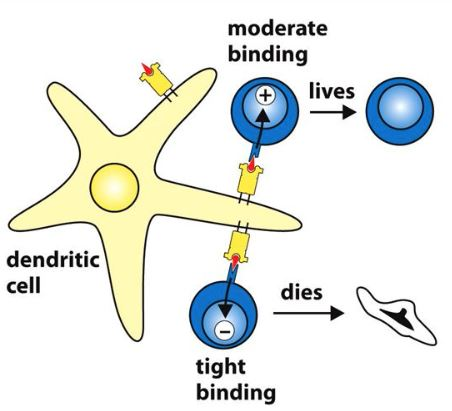
\includegraphics[width=0.6\textwidth]{NSA/figures/NST.JPG}
  \caption{Negative selection of T cells}
  \end{figure}
\end{frame}

\begin{frame}{Biological immune system}
  \begin{figure}[hb]
  \centering
  %\includegraphics[width=0.6\textwidth]{NSA/figures/is.jpg}
  \caption{Antigen-antibody interaction}
  \end{figure}
\end{frame}

% You can reveal the parts of a slide one at a time
% with the \pause command:
\begin{frame}{Defining the NSA}
  \begin{itemize}
  \item<1->{
    Define Self as a normal pattern of activity or stable behavior of a system/process.\\
    -Represent the collection as multiset of S of strings of length \emph{l} over a finite alphabet.
  }
  \item<2-> {   
    Generate a set R of detectors,each of which fails to match any string in S.
  }
  % You can also specify when the content should appear
  % by using <n->:
  
  \end{itemize}
\end{frame}
 
\begin{frame}{Flowchart}
  \begin{figure}[hb]
  \centering
  %\includegraphics[width=0.8\textwidth]{NSA/figures/flowchart1.jpg}
  \caption{Generation of effective detector}
  \end{figure}
\end{frame}

\begin{frame}{Defining the NSA}
  \begin{itemize}
  \item {
    Monitor new observations for changes by continually testing the detectors matching against representatives of S.  If any detector ever matches, a change must have occurred in system behavior.
  }
  \end{itemize}
\end{frame}

\begin{frame}{Flowchart}
  \begin{figure}[hb]
  \centering
  %\includegraphics[width=0.8\textwidth]{NSA/figures/flowchart2.jpg}
  \caption{Self-monitoring}
  \end{figure}
\end{frame}

\section{Immune Network Theory}

\begin{frame}
\Huge \textbf{Immune Network Theory}
\large {Shi,Haixin}
\end{frame}

\begin{frame}{Immune Network Theory}{Jerne's idiotypic network hypothesis}
  \begin{itemize}
  \item \large{
    Immunologists in the early 1970's were in the process of discovering a wealth of information about how the immune system worked.
  }
  \item \large{
    Jerne's network hypothesis was a radical innovation, which states that the regulation of the adaptive immune system involves interactions between V regions.
  }
  \end{itemize}
\end{frame}

\begin{frame}{Immune Network Theory}{Jerne's idiotypic network hypothesis}
   \begin{itemize}
   \item \large
    Jerne introduced three terms:
    \begin{itemize}
    \item
      \large{\textcolor{red}{epitope} (antigenic determinant): the part of an antigen that is recognized by the immune system.}
    \item
      \large{\textcolor{red}{idiotope}: the unique set of antigenic determinants (epitopes) of the variable portion of an antibody.}
    \item
      \large{\textcolor{red}{paratope} (antigen-binding site): is a part of an antibody which recognizes and binds to an antigen.}
    \end{itemize}
  \end{itemize}
\end{frame}

\begin{frame}{Immune Network Theory}{Dualisms}
   \begin{itemize}
   \item \large
    two main kinds of cells:
    \begin{itemize}
    \item
      \large{T cells}
    \item
      \large{B cells}
    \end{itemize}
   \item \large
    two main kinds of interactions:
    \begin{itemize}
    \item
      \large{stimulation}
    \item
      \large{suppression}
    \end{itemize}
  \end{itemize}
\end{frame}

\begin{frame}{Immune Network Theory}{Jerne's model of the network}
  \begin{itemize}
  \item \large
     The network was proposed by Jerne in 1973.
  \end{itemize}
  \par
  \centering
    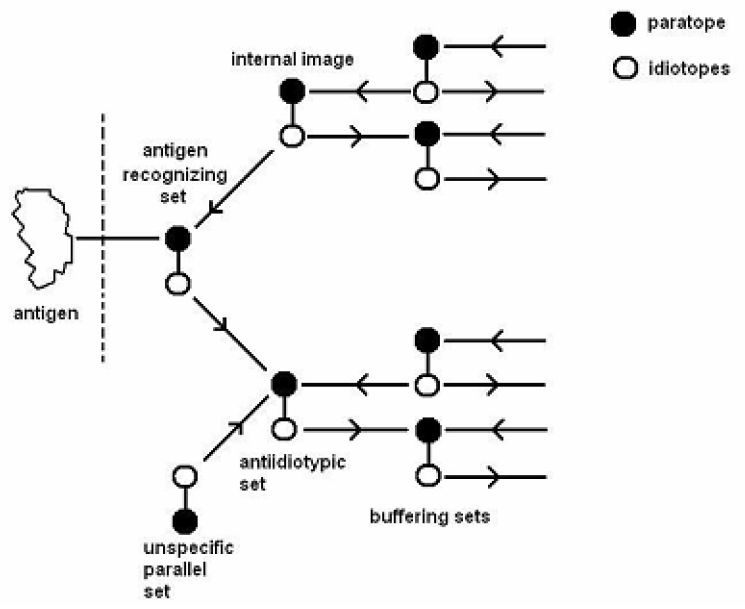
\includegraphics[scale=0.5] {img/network_model_jerne.png}
  \par
\end{frame}

\begin{frame}{Immune Network Theory}{The first mathematical model}
  \begin{itemize}
  \item \large
     The formula describes the dynamics of a typical clone consisting of L cells (lymphocytes):
  \end{itemize}
  \begin{equation} \large{
     \frac{dL}{dT}= \alpha -\beta L+\sum_{i=1}^{N}\varphi (E_{i},K_{i},t)-L\sum_{j=1}^{n}\psi (I_{j},K_{j},t)}
  \end{equation}
\end{frame}

\begin{frame}{Immune Network Theory}{Limitations of the Jerne model}
  \begin{itemize}
  \item \large
   While Jerne's model was a huge conceptual advance, he candidly recognized it's
   limitations:
   \begin{columns}[c] 
    \column{.45\textwidth} 
    \begin{itemize}
    \item \large{(a)Simplicity}
    \item \large{(b)Scope}
    \item \large{(c)Predictions}
    \item \large{(d)Resolution of Paradoxes}
    \end{itemize}
    \column{.55\textwidth} 
    \begin{itemize}
    \item \large{(e)Mechanistic basis}
    \item \large{(f)Rigour}
    \item \large{(g)Robustness}
    \item \large{(h)Aesthetics}
    \end{itemize}
    \end{columns}
  \end{itemize}
\end{frame}

\begin{frame}{Immune Network Theory}{The Richter theory}
  \begin{itemize}
  \item \large
     The network was thus simplified from Jerne's two-dimensional network to a one dimensional chain.
  \end{itemize}
  \par
  \centering
    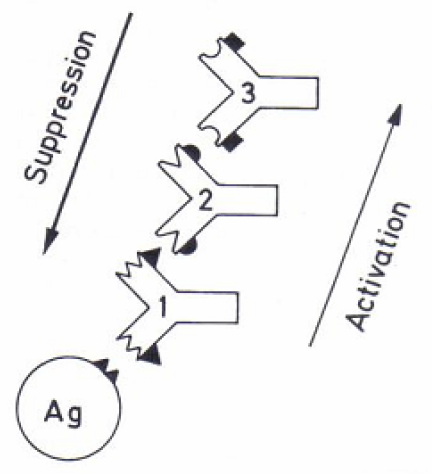
\includegraphics[scale=0.5] {img/network_model_richter.png}
  \par
\end{frame}

\begin{frame}{Immune Network Theory}{Modes of response}
  \begin{itemize}
  \item \large
     Low dose tolerance in the Richter model.
  \end{itemize}
  \par
  \centering
    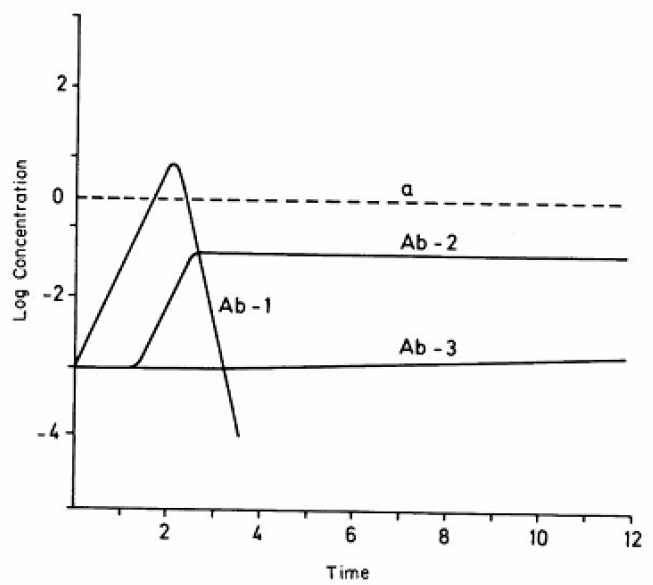
\includegraphics[scale=0.5] {img/low_dose_tolerance.png}
  \par
\end{frame}

\begin{frame}{Immune Network Theory}{Modes of response}
  \begin{itemize}
  \item \large
     The immune response in the Richter model.
  \end{itemize}
  \par
  \centering
    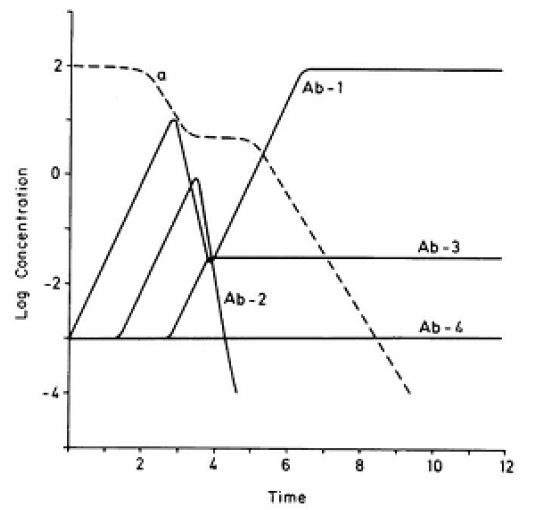
\includegraphics[scale=0.5] {img/immune_response.png}
  \par
\end{frame}

\begin{frame}{Immune Network Theory}{Modes of response}
  \begin{itemize}
  \item \large
     High dose tolerance in the Richter model.
  \end{itemize}
  \par
  \centering
    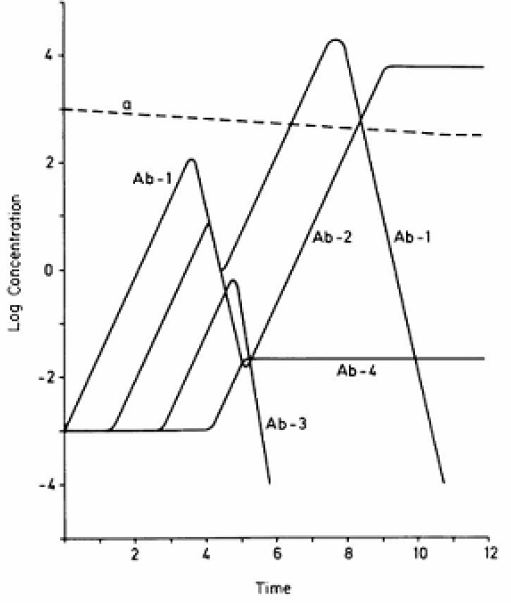
\includegraphics[scale=0.5] {img/high_dose_tolerance.png}
  \par
\end{frame}

\begin{frame}{Immune Network Theory}{Modes of response}
  \begin{itemize}
  \item \large
    The improved network model which adds inhibitory interactions.
  \end{itemize}
  \par
  \centering
    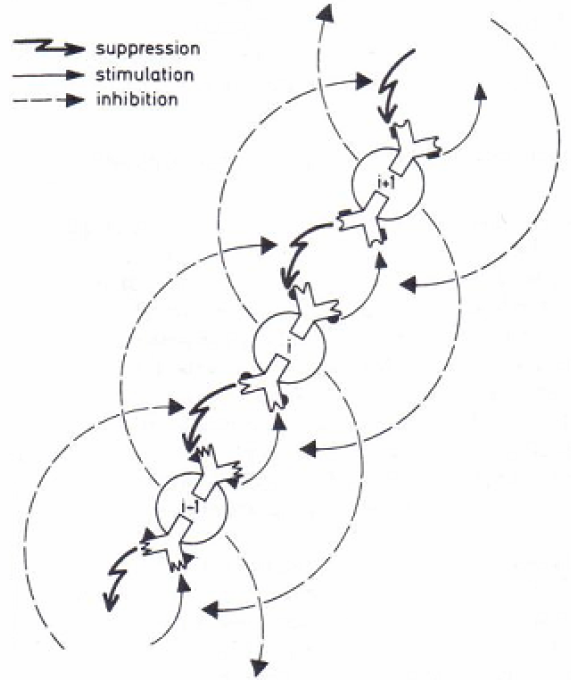
\includegraphics[scale=0.4] {img/Improved_network_model.png}
  \par
\end{frame}

\begin{frame}{Immune Network Theory}{Richter's mathematical model}
  \begin{itemize}
  \item \large
    Richter translated the above ideas into differential equations, and pictures above can be obtained by integrating his equations:
  \end{itemize}
  \begin{equation} \large{
    \frac{dS_{i}}{dt}=\frac{1}{\tau _{b}}f(S_{i-1},S_{i},S_{i+1})S_{i}-\frac{1}{\tau _{d}}g(S_{i-1},S_{i},S_{i+1})S_{i}}
  \end{equation}
\end{frame}

\begin{frame}{Immune Network Theory}{Achievements of the Richter theory}
  \begin{itemize}
  \item \large{
    It showed that Jerne's network concept could be reduced to manageable proportions.
  }
  \item \large{
    The Richter theory showed that there are three basic types of specific interactions which are important for such models - stimulation, inhibition (blocking) and elimination (killing).
  }
  \item \large{
    It illustrated a potential importance of thresholds in stabilizing the immune system.
  }
  \end{itemize}
\end{frame}

\begin{frame}{Immune Network Theory}{The symmetrical network theory}
  \begin{itemize}
  \item \large
    The symmetrical network theory incorporates symmetric interactions between idiotypes and antiidiotypes.
  \end{itemize}
  \par
  \centering
    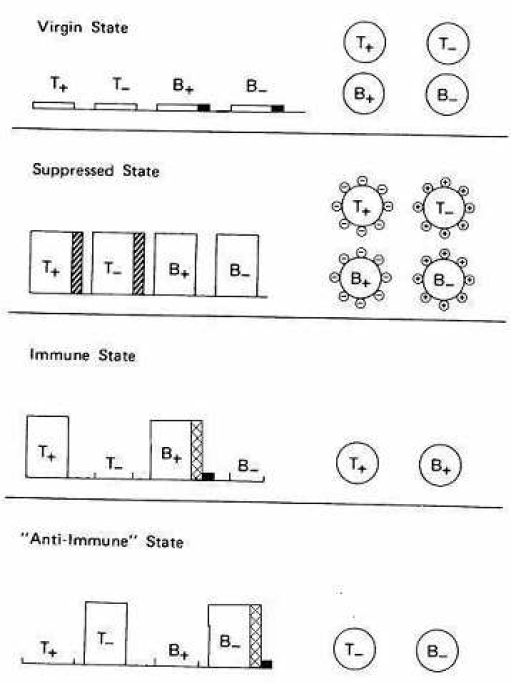
\includegraphics[scale=0.40] {img/symmetrical_network_theory.png}
  \par
\end{frame}

\begin{frame}{Immune Network Theory}{The environmental detection algorithm}
  \begin{itemize}
  \item \large{
    The movement direction of robot:
  }
  \end{itemize}
  \par
  \centering
    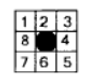
\includegraphics[scale=0.8] {img/movement_direction.png}
  \par
  \begin{itemize}
  \item \large{
    The antigen information of robot:
  }
  \end{itemize}
  \begin{equation} \large{
     g_{i}=\frac{1}{(k_{1}\cdot expense+k_{2}\cdot occupy+k_{3}\cdot gain+1)}}
  \end{equation}
\end{frame}

\begin{frame}{Immune Network Theory}{The environmental detection algorithm}
  \begin{itemize}
  \item \large{
    The interaction between robotic antibodies:
  }
  \end{itemize}
  \par
  \centering
    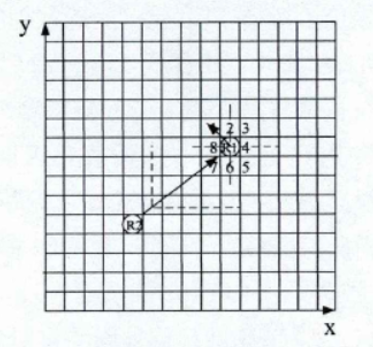
\includegraphics[scale=0.6] {img/immune_network_force_diagram.png}
  \begin{equation} \large{
     \overline{R_{2}R_{1}}=\overline{(x_{2}-x_{1})(y_{2}-y_{1})}}
  \end{equation}
\end{frame}

\begin{frame}{Immune Network Theory}{The environmental detection algorithm}
  \centering
    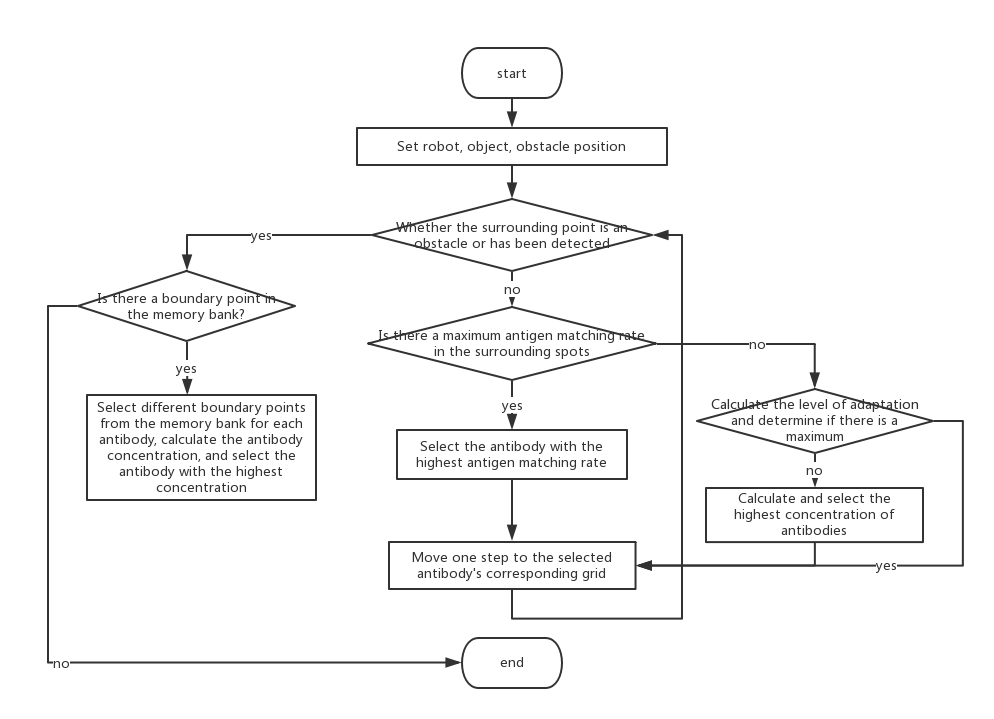
\includegraphics[scale=0.30] {img/immune_network_flowchat.png}
\end{frame}

\begin{frame}{Immune Network Theory}{The environmental detection algorithm}
  \centering
    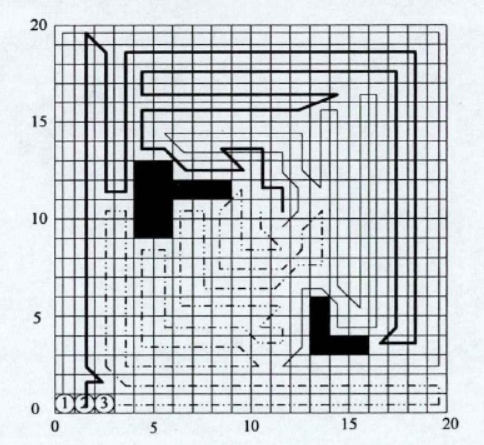
\includegraphics[scale=0.70] {img/immune_network_route_map.png}
\end{frame}




\section{Artificial Immune Network}

\begin{frame}
\huge \textbf{{Artificial Immune Network(AIN)}}
\large {Zhong,Wenfeng}
\end{frame}

\begin{frame}{What is AIN?}
\begin{itemize}
\item {\textbf{The artificial immune network model(AIN)} regards artificial immune system(AIS) as a network structure composed of nodes (lymphocytes). Through the information transfer and interaction between nodes, the immune system functions such as recognition, response, and memory are achieved.}
\item {\textbf{applied to} data mining , time series prediction, pattern recognition, optimization, fault detection ...}
\end{itemize}
\end{frame}

\begin{frame}{Features}
\begin{itemize}
\item Realize and express the results of data information processing in the form of a network;
\item Deal with large amounts of data in decentralized organizations;
\item Achieve sustainable learning in the form of a dynamic network;
\item Threshold-based information processing;
\item Quickly process data information in a parallel, distributed manner.
\end{itemize}
\end{frame}

\begin{frame}{Relationship of AIN Models}
\begin{center}
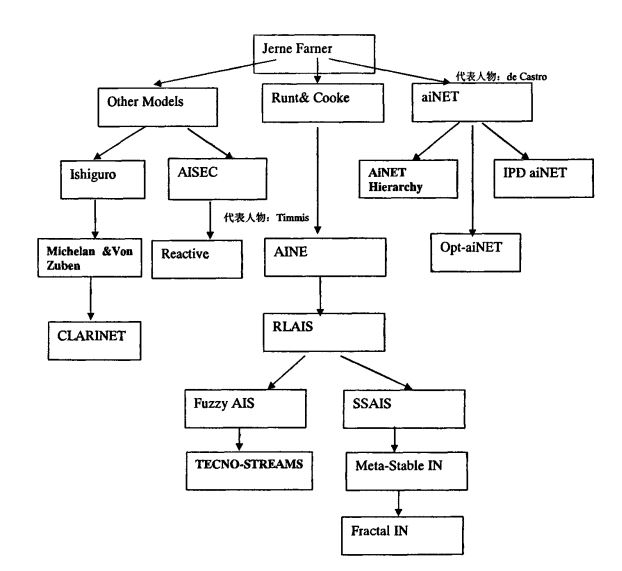
\includegraphics[scale=0.64]{img/relationship_of_AIN.JPG}
\end{center}
\end{frame}


\begin{frame}{Basic framework of AIN}
\begin{center}
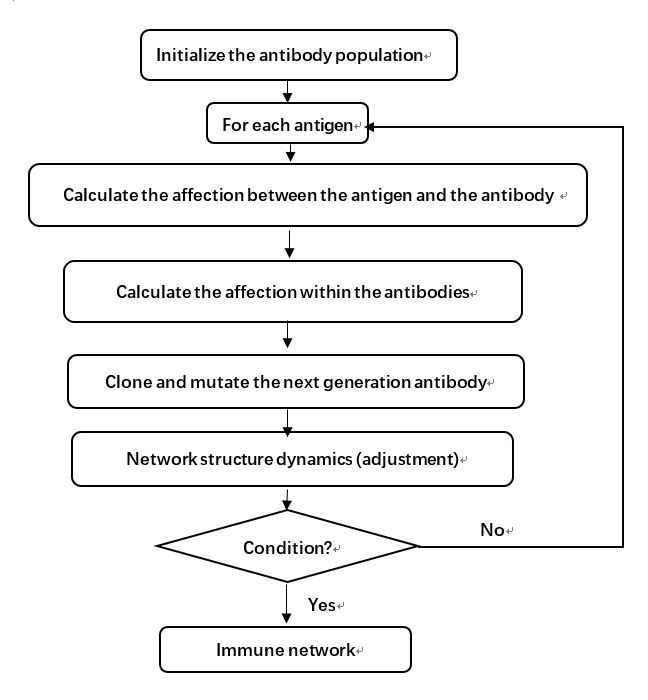
\includegraphics[scale=0.55]{img/basic_framework_of_AIN.JPG}    
\end{center}
\end{frame}

\begin{frame}{Applications of AIN}{multimodal function optimization}
\begin{columns}[c] 
\column{.5\textwidth} 
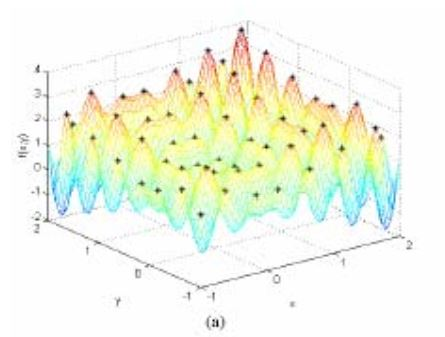
\includegraphics[scale=0.6]{img/multimodal_function_optimization_AIN.JPG}
\column{.5\textwidth} 
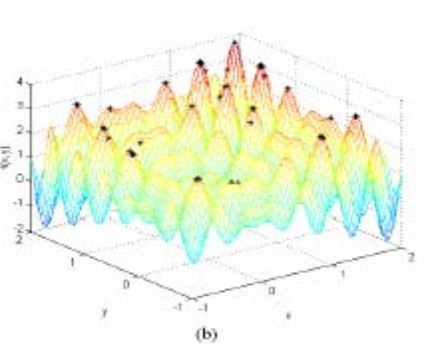
\includegraphics[scale=0.6]{img/multimodal_function_optimization_clonalg.JPG}
\end{columns}
\end{frame}

\begin{frame}{Applications of AIN}{associative classification}
\begin{columns}[c] 
\column{.5\textwidth} 
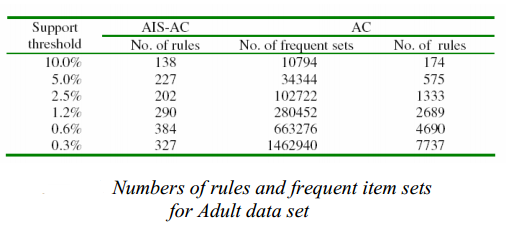
\includegraphics[scale=0.45]{img/associative_classification_table.png}
\column{.5\textwidth} 
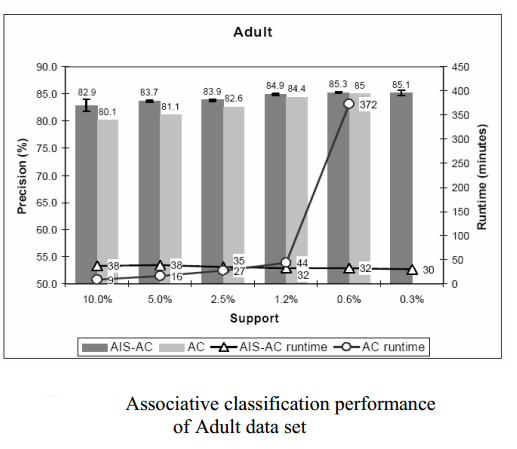
\includegraphics[scale=0.3]{img/associative_classification_figure.png}
\end{columns}
\end{frame}


\begin{frame}
\centering \Huge \textbf{Thank You!}
\end{frame}

\documentclass{beamer}

\usetheme{Madrid}
\usepackage{indentfirst} 
\usepackage{graphicx} 
\usepackage{booktabs}
\usepackage{amsmath}
\allowdisplaybreaks[4]
\title{Hybrid Immune Algorithm}


\subtitle{}

\author{2017Spring OPT}

\institute[] 
{Han,Shiqi}

\date{\today}

\subject{Theoretical Computer Science}

\begin{document}

\begin{frame}
  \titlepage
\end{frame}

\begin{frame}{Why Hybrid?}
\begin{itemize}
\item {\textbf{No Free Lunch Theorem}\\ \footnotesize{--- David Wolpert \& William Macready}}
\item {\textbf{Hybridize Where Possible}\\ \footnotesize{--- L. D. Davis}}
\end{itemize}
\begin{block}
\small{In the limited search space, for the iterative optimization algorithm, there is no algorithm that is best for all problems. Different optimization algorithms have different application advantages and disadvantages, and there is a complementarity between the algorithms.}
\end{block}
\end{frame}

\begin{frame}{Hybrid Ways}
\begin{columns}[c] 
\column{.45\textwidth} 
\begin{itemize}
\item {Operator Transplantation}
\item {Operator Series}
\item {Operator Competition}
\end{itemize}
\column{.55\textwidth} 
\includegraphics[height=3cm]{img/img1.jpg}
\end{columns}
\end{frame}

\begin{frame}{Hybrid Immune Algorithm}
\begin{itemize}
\item{Immune Genetic Algorithm}
\item{Immune Particle Swarm Optimization}
\item{Synergetic Evolutionary Immune Algorithm}
\item{Immune Ant colony algorithm}
\item{
Quantum Immune Algorithm\\
Chaotic Immune Algorithm\\
Fuzzy Immune System\\
Immune Neural Network Algorithm\\
......
}
\end{itemize}
\small
{\noindent

}
\end{frame}

\begin{frame}{Immune Ant Colony Algorithm}{Ant Colony Algorithm}
 \large \textbf{Ant Colony Algorithm}\\~\\
 \small
 {
Ants leave a \textcolor{red}{pheromone} in the path that it travels when foraging, and can feel the intensity of it during the movement and tend to move in the direction of \textcolor{red}{high concentration}, so the  group behavior will show \textcolor{red}{positive feedback} with pheromone information.
 }\\
\end{frame}

\begin{frame}{Immune Ant Colony Algorithm}{Problems and Solving}
\begin{table}
\begin{tabular}{p{11em}|p{19em}}
\toprule
\textbf{Ant Colony Weakness} & \textbf{Immune Algorithms Advantages}\\
\midrule \small
\footnotesize{Lack of information at first, convergence slows} & \footnotesize{ \textcolor{red}{Clone mutation mechanism}, use affinity describe the matching between antibody and antigen, fast global search capabilities}\\
\footnotesize{Easy to fall into local extreme point and premature convergence occurs} & \footnotesize{ \textcolor{red}{Concentration inhibition mechanism}, influencing road path selection probability to maintain the ant colony diversity} \\
\bottomrule
\end{tabular}
\end{table}
\end{frame}

\begin{frame}{Immune Ant Colony Algorithm}{TSP}
 \large \textbf{Traveling Salesman Problem}\\~\\
 {TSP is a \textcolor{red}{shortest path problem}. For n cities, choose any cities as the starting point and traverse all the cities back to the starting point. When the sum of the paths is the \textcolor{red}{shortest}, the path is optimal.}
 \begin{equation} \small{
 T_{d}=\sum_{i=1}^{n-1}d\left (v_{i},v_{i+1}\right )+d\left (v_{1},v_{n} \right)}
 \end{equation}
\end{frame}

\begin{frame}{Immune Ant Colony Algorithm}{Term Definition}
\large \textbf{Term Definition}\\~\\
\begin{itemize}
\item \textbf{Antigen}
\item \textbf{Antibody}
\begin{equation}\small{
  D=\left \{\left \langle s,T_d\right \rangle | s \in P , T_d \in N \right \}}
\end{equation}
\item \textbf{Affinity}
\small{
\begin{equation}
  f_{dist}\left(A_{b},A_{g} \right) = 1 /\left(A_{b}.dist - A_{g}.dist\right)
\end{equation}
\begin{equation}
  T = \left(\sum_{i=1}^{n} \sum_{j=1}^{n}d\left(i,j\right)\right)/\left(2n\right)
\end{equation}
\begin{equation}
  f_{dist}\left(A_{b},A_{g} \right) = 1 /\left(A_{b}.dist - T\right)
\end{equation}}
\end{itemize}
\end{frame}

\begin{frame}{Immune Ant Colony Algorithm}{Term Definition}
\large \textbf{Term Definition}\\~\\
\begin{itemize}
\item \textbf{Memory Cells}
\begin{equation} \small{
  M=\left \{ x |f_{dist} \left(A_{b},A_{g}\right)\geqslant \theta,x \in D \right \}}
\end{equation} \small{
\item \textbf{Path Transition Probability}}
\begin{equation}
p{_{ij}}^{k} =
\begin{cases}
\frac{[\tau_{ij}(t)]^\alpha \cdot [\eta_{ij}]^\beta} { \sum\limits_{s \subset allowed_{k}} [\tau_{is}(t)]^\alpha \cdot [\eta_{is}(t)]^\beta} & j \in allowed_k \\
0 & else
\end{cases}
\end{equation}
\end{itemize}
\end{frame}

\begin{frame}{Immune Ant Colony Algorithm}{Algorithms Step}
\large \textbf{Step 1} \normalsize{Calculate a feasible solution using immune algorithm}\\~\\
\begin{itemize}
\item{Enter question and determine the antibody encoding}
\item{Calculate antibody affinity $f_{dist}$, Memory cell $M(f_{dist}\geqslant\theta)$}
\item{Antibody clone variation \qquad $A_{bj}\rightarrow C_j \rightarrow C_j^*$}
\begin{equation}\small{
i=INT[num \times \beta \div con]}
\end{equation}
\begin{equation}\small{
con_i=\frac{M_{bi}}{M_{b}} }
\end{equation}
\item{Update group \qquad \small{$f_{dist}(A_{bj}^*,A_{gj}) > f_{dist}(A_{bj},A_{gj}) ?$}} 
\item{Terminal condition}
\end{itemize}
\end{frame}

\begin{frame}{Immune Ant Colony Algorithm}{Algorithms Step}
\large \textbf{Step 2} \normalsize {Initialize the pheromone based on feasible solution}\\~\\
\begin{equation}
\tau_{ij}(0)=
\begin{cases}
\tau_C +\tau_G & e_{ij} \in L^* \\
\tau_C & else
\end{cases}
\end{equation}
\begin{equation}
\tau_G = \frac{Q}{L^*}
\end{equation}
\centering \small{
{$\tau$:pheromone amount}\\ {$Q$: a cycle pheromone amount}\\ {$L^*$:optimal path length}
}
\end{frame}

\begin{frame}{Immune Ant Colony Algorithm}{Algorithms Step}
\large \textbf{Step 3} \normalsize {Construct probability formula using immune inhibition operators}\\~\\
\centering \small { \textcolor{red}{Path Concentration $C_{ij}$:} the amount of ants that choose path $e_{ij}$}
\begin{equation}\small{
C_{ij}(t) = \frac{1}{M} \sum\limits_{k=1}^{M}iif \left(e_{ij} \in Tour^k(t),1,0\right)}
\end{equation}
\begin{equation}\small{
C_{ij}^k(t) = \frac{1}{M} \sum\limits_{k=1}^{k-1}iif \left(e_{ij} \in Tour^k(t),1,0\right)}
\end{equation}
\end{frame}

\begin{frame}{Immune Ant Colony Algorithm}{Algorithms Step}
\large \textbf{Step 3} \normalsize {Construct probability formula using immune inhibition operators}\\~\\
\centering \small {Update pheromone amount $\tau_{ij}$ considering path concentration $c_{ij}$}
\begin{equation}
\tau_{ij}^k(t)=
\begin{cases}
\tau_{ij} \cdot \left(\lambda \cdot c_{ij}^k(t)\right) & if \quad c_{ij}^k(t) > c_0 \\
\tau_{ij} & else
\end{cases}
\end{equation}
\begin{equation}
p{_{ij}}^{k} =
\begin{cases}
\frac{[\tau_{ij}^k(t)]^\alpha \cdot [\eta_{ij}]^\beta} { \sum\limits_{\mu \subset N^k_l(t)} [\tau_{i\mu}^k(t)]^\alpha \cdot [\eta_{i\mu}(t)]^\beta} & if j \in N^k_i(t) \\
0 & else
\end{cases}
\end{equation}
\end{frame}

\begin{frame}{Immune Ant Colony Algorithm}{Algorithms Step}
\large \textbf{Step 4} \normalsize {Update pheromones}\\~\\
\begin{equation} \small{
\tau_{ij}(t+n) = (1-\omega)\cdot\tau_{ij}(t)+\omega\cdot C}
\end{equation} \\~\\
\centering \small {Update the pheromone of shortest path and longest path}
\begin{equation}\small{
\tau_{ij}(t+n) = (1-\rho)\cdot\tau_{ij}(t)+\rho\cdot \Delta{\tau_{ij}}'(t)}
\end{equation}
\begin{equation} \small{
\Delta{\tau_{ij}}'(t) = 
\begin{cases}
\frac{Q}{L_{best}} & e_{ij} \in L_{best} \\
-\frac{Q}{L_{worst}} & e_{ij} \in L_{worst} \\
0 & else
\end{cases}}
\end{equation}
\end{frame}

\begin{frame}{Summary}
\textbf{Two tyeps of Hybrid Immune Algorithms} \\~\\
\begin{itemize}
\item{Introduce the immune concept and mechanism into other algorithms, overcome local extreme points and improve convergence accuracy}
\item{Introduce other algorithms into immune algorithm, increase the convergence speed of algorithm}
\end{itemize}
\end{frame}

\begin{frame}
\centering \Huge \textbf{Thank You!}
\end{frame}
\end{document}


\end{document}


